\chapter{The Linear Paul Trap}
\label{chap:LinTrap}

\section{Single ion in a linear Paul Trap}
\label{sec:1Ion}
The linear Paul trap consists of four rods, each of which is split into three electrodes as is seen on \cref{fig:PaulTrap}. The coordinate system for the trap is defined such that the $z$-axis runs down along the centre of the trap,
while the $x,y$-axes go between diagonally opposed rods. Furthermore we define $z_0$ to be half the length of center electrodes, while we define $r_0$ as half the distance between diagoanlly opposed electrodes as seen on \cref{fig:PaulTrap}.
\begin{figure}
    \centering
    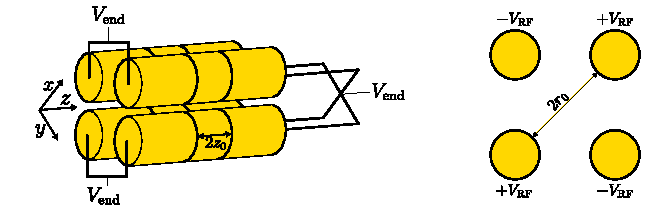
\includegraphics{main/Paul_Trap.pdf}
    \caption{Example schematic of a linear paul trap showing: (left) a 3D model of the paul Trap with both the DC endcap voltages applied.
    (right) an end-view down the Paul trap, showing the phase of the RF voltages applied to the different rods.}
    \label{fig:PaulTrap}
\end{figure}
In order to trap an ion along the $z$-direction a static voltage $V_{end}$ is applied to all of the electrodes on the end of the rods. By applying such a votlage to these endcap electrodes an electrical potential is generated, which in the region around the centre of the trap can be written as
\begin{equation}
    \phi_{DC}(z) = \frac{\kappa V_{end}}{z_0^2}z^2,
    \label{eq:phi_DC_z} 
\end{equation}
where $\kappa$ is a constant defined by the specific geometry of the trap, and $z$ is the position of the ion along the $z$ axis.
Thus an ion of mass $m$ and charge $Q$ finds itself sitting in a harmonic potential
\begin{equation}
    \label{eq:omega_z}
    V_{DC}(z) = \frac{1}{2}m\omega_z^2 z^2, \quad\omega_z = \sqrt{\frac{2Q\kappa V_{end}}{mz_0^2}},
\end{equation}
where $\omega_z$ is the frequency of the ions oscillating motion along the $z$-axis.

For the radial directions it is necessary to take a slightly different approach, indeed Earnshaw's theorem \textcolor{red}{Earnshaw} states
that it is impossible to trap a charged particle in all three directions, solely through the use of electrostatic forces. If we look at the electrical potential in the $x,y$-plane from the DC endcaps we also find
\begin{equation}
    \phi_{DC}(x,y) = -\frac{\kappa V_{end}}{2z_0^2}(x^2+y^2),
\end{equation}
which is clearly repulsing the ion from the center of the trap.

To counteract this repulsive effect, we employ an RF voltage, oscillating at frequency $\Omega_{RF}$, with an amplitude $V_{RF}$ on all four rods. Neighbouring rods have opposites phases while, dioganlly opposing rods share a phase, as seen on \cref{fig:PaulTrap}.
We can then write the total time dependant electrical potential in the $x,y$-plane as \textcolor{red}{KARIN}
\begin{equation}
    \phi(x,y,t) = -\frac{\kappa V_{end}}{2z_0^2}(x^2+y^2)-\frac{V_{RF}}{2r_0^2}(x^2-y^2)\cos{(\Omega_{RF}t)},
\end{equation}
where the first term comes from the repulsing DC potential, and the second term comes from the RF voltages applied to the rods.

The equations of motion in the radial plane can be rewritten on a more compact form by adopting the notation
\begin{equation}
    \tau = \frac{\Omega_{RF}t}{2},\quad a = -\frac{4Q\kappa V_{DC}}{mz_0^2\Omega_{RF}^2},\quad q_x = -q_y = 
    \frac{2QV_{RF}}{mr_0^2\Omega_{RF}^2},
\end{equation}
which allows for the equations of motion to be written as
\begin{equation}
    \frac{\text{d}^2\gamma}{\text{d}\tau^2} + (a-2q_\gamma\cos{(2\tau)})\gamma,\quad \gamma\in\{x,y\}
    \label{eq:Mathieu}.
\end{equation}
\Cref{eq:Mathieu} is known as the Mathieu equation \textcolor{red}{CITE}, the Mathieu equation has bounded solutions for several sets of $(a,q_\gamma)$ parameters,
however, the conditions usually used in experiment state that for a given value of $q_\gamma$, $a$ must be found between the two curves approximated by \textcolor{red}{CITE}
\begin{align}
    &a_0(q_\gamma) \approx -\frac{1}{2}q_\gamma^2 +\frac{7}{128}q_\gamma^4 -\frac{29}{2304}q_\gamma^6+\frac{68687}{18874368}q_\gamma^8,\\
    &b_1(q_\gamma) \approx 1-q_\gamma-\frac{1}{8}q_\gamma^2+\frac{1}{64}q_\gamma^3-\frac{1}{1536}q_\gamma^4-\frac{11}{36864}q_\gamma^5.
\end{align}
Together these two lines form what is known as a stability diagram. Since a positive DC voltage is needed for the confinement in the axial direction, we usually confine ourselves to considering stability in the $a<0$ region. A plot of the stable region for the linear Paul trap can be see on \cref{fig:Stability1}
\begin{figure}
    \centering
    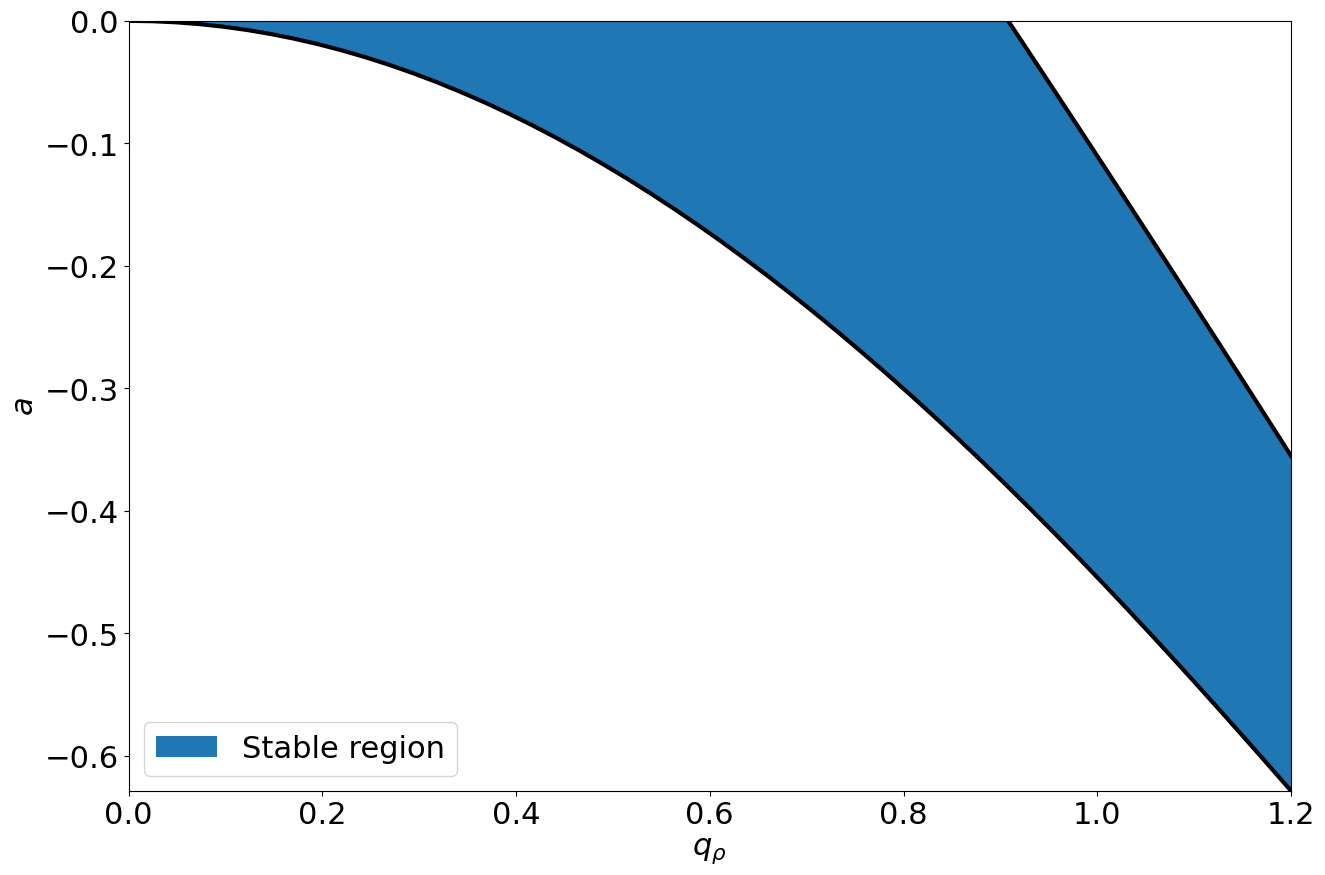
\includegraphics[width =0.8\textwidth]{main/Stability.png}
    \caption{Plot of the Mathieu stability diagram for negative values of $a$. The blue colored area contains the set of bounded, and thus stable solution to the Mathieu equation of \cref{eq:Mathieu}}
    \label{fig:Stability1}
\end{figure}

In the case where $\vert a\vert,\vert q_\gamma\vert\ll 1$ the solution to \cref{eq:Mathieu} can be approximated to
\begin{equation}
    \label{eq:omega_r}
    \gamma(t) = \gamma_0\bigg(1-\frac{q_\gamma}{2}\cos{(\Omega_{RF}t)}\bigg)\cos{(\omega_r t)},\quad \omega_r = \frac{\Omega_{RF}}{2}\sqrt{\frac{q_\gamma^2}{2}+a}.
\end{equation}
Since $\vert q_\gamma\vert\ll 1$ we see that there is a large-amplitude motion of the ion at frequency $\omega_r$. This motion is typically referred to as secular motion in the litterature. The frequency $\omega_r$ is much slower than the RF frequency of the trap (typically 10's-100's of kHz vs. 5MHz in the case of our trap). 

In addition there is a small-amplitude motion superimposed on top, oscillating at the RF frequency. This motion is typically referred to as micromotion. Thus the full picture we now get, is one of the ion performing slow, but large oscillations in the radial plane, with an additional micromotion on top. An example trajectory can be seen on \cref{fig:micromotion}, where the micromotion is clearly visible.



\begin{figure}
    \centering
    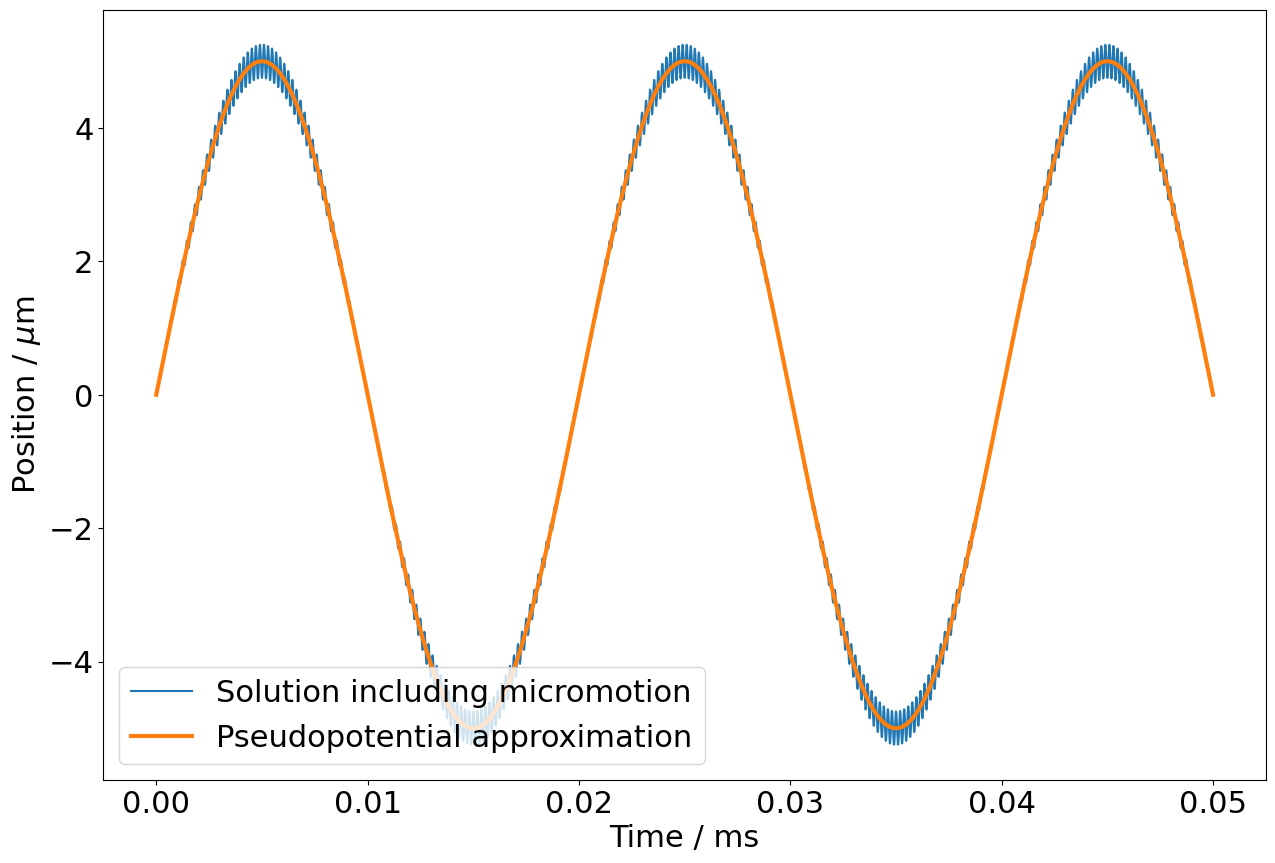
\includegraphics[width = 0.8\textwidth]{main/Micromotion.png}
    \caption{Trajectories including (blue) micromotion or calculated through the pseudopotential approximation (orange), for $\gamma_0 = 5 {\mu}$m, $\omega_r = 2\pi\times 50$kHz, $\Omega_{RF} = 2\pi\times 5.2$MHz.}
    \label{fig:micromotion}
\end{figure}

It is common to average over the micromotion of the ion, keeping only the term oscillating at $\omega_r$. If this is done, it is clear that the ion then moves as if in an effective potential (often referred to as pseudopotential in the litterature) given by
\begin{equation}
    V_{Pseudo}(\gamma) = \frac{1}{2}m\omega_r^2\gamma^2,\quad \gamma\in\{x,y\}.
\end{equation}
The pseudopotential approximation is especially useful when working with trapped ions in a quantum mechanical regime, since their Hamiltonian is then simply that of a harmonic oscillator, which is one of the most well-studied examples in all of quantum mechanics.
\section{Two ions in a linear Paul trap}
We now move on to the topic of two co-trapped ions in a Paul trap. We shall denote the ions 1 and 2 respectively, with masses $m_1,m_2$, and charges $Q_1,Q_2$.
Remembering to include the Coulomb interaction between the two ions, the potential energy of the system, in the pseudopotential approximation, can then be written as
\begin{align}
    \nonumber V(\vec{r_1},\vec{r_2}) = &\frac{1}{2}m_1\bigg(\omega_{1,z}^2z_1^2+\omega_{1,r}^2(x_1^2+y_1^2)\bigg)+\frac{1}{2}m_2\bigg(\omega_{2,z}^2+\omega_{2,r}^2(x_2^2+y_2^2)\bigg)\\
    & +\frac{Q_2Q_2}{4\pi\epsilon_0}\frac{1}{\vert r_1-r_2\vert},
    \label{eq:fullV}
\end{align}
where $\omega_{j,(r/z)}$ is calculated as in \cref{eq:omega_r,eq:omega_z}, using the mass and charge of ion $j$.
For the rest of the derivations in this report we are, unless otherwise noted, going to ignore the $y$ part of motion of the ions since our system exhibits a radial symmetry, and thus any equations that hold for $x$ will hold for $y$ as well.

We shall first derive the equilibrium positions for the two ions. Assuming the radial trapping is stronger than the axial trapping we know that the ions will along themselves along the $z$-axis, and thus we slightly simplify the potential to be minimized
\begin{equation}
    V(z_1,z_2) = \frac{1}{2}m_1\omega_{1,z}^2z_1^2 + \frac{1}{2}m_2\omega_{2,z}^2z_2^2 + \frac{Q_1Q_2}{4\pi\epsilon_0}\frac{1}{z_1-z_2},
\end{equation}
where we assume without loss of generality that $z_1>z_2$. Taking the derivatives with respect to the ion coordinates to be zero we find
\begin{align}
    &\frac{\partial V}{\partial z_{1}} = m_1\omega_{1,z}^2z_{1,eq} - \frac{Q_1Q_2}{4\pi\epsilon_0}\frac{1}{(z_{1,eq}-z_{2,eq})^2}  = 0\label{eq:derivativeZ1},\\
    &\frac{\partial V}{\partial z_{2}} = m_2\omega_{2,z}^2z_{2,eq} + \frac{Q_1Q_2}{4\pi\epsilon_0}\frac{1}{(z_{1,eq}-z_{2,eq})^2} = 0,
\end{align}
where the $(eq)$ subscript denotes the value is taken at the equilibrium position. Adding the two together we find
\begin{equation}
    z_{1,eq} = -\rho z_{2,eq},
\end{equation}
where $\rho = \frac{Q_2}{Q_1}$ is the charge ratio between the two ions. It is interesting to note that the equilibrium positions are entirely independent on the masses of the ions.
We can now plug this relationship back into \cref{eq:derivativeZ1} to find an expression for $z_{1,eq}$
\begin{equation}
    z_{1,eq} =\bigg(\frac{Q_1Q_2}{4\pi\epsilon_0m_1\omega_{1,z}^2}\frac{1}{(1+\frac{1}{\rho})^2}\bigg)^{1/3},
\end{equation}
it has to be noted that if one expands the $\omega_{1,z}$ factor in the denominator one finds that the equilibrium position is mass independent. This has not been done here, as it lengthens the expression considerably.

In this derivation we assumed that the ions aligned themselves along the $z$-axis, which is also the desired case. However one of course has to design any experiment such that the voltages applied result in such an orientation. This leads to further "stability" requirements for the two-ion system.
Following the derivation above one can similarly find expressions for equilibrium positions along the $x$-axis. The ions will naturally align themselves along the axis which has the lowest energy at equilibrium. Through much massaging, one finds, that if the ions are to align along $z$, the follow inequality must hold:
\begin{equation}
    \frac{m_1m_2\omega_{1,z}^2\omega_{2,z}^2}{m_1\omega_{1,z}^2+m_2\omega_{2,z}^2} < \frac{m_1m_2\omega_{1,r}^2\omega_{2,r}^2}{m_1\omega_{1,r}^2+m_2\omega_{2,r}^2}.
\end{equation}
In addition to this, the ions must also uphold the stability criterium outlined in \cref{sec:1Ion}. Given that both ions need to be stable \textit{and} trapped along the $z$-axis the new stability diagram can look considerably different. An example for a polyporphyrin of mass 9000amu and charge 24e trapped alongside Ba$^+$ is seen on \cref{fig:Stability2}.
\begin{figure}
    \centering
    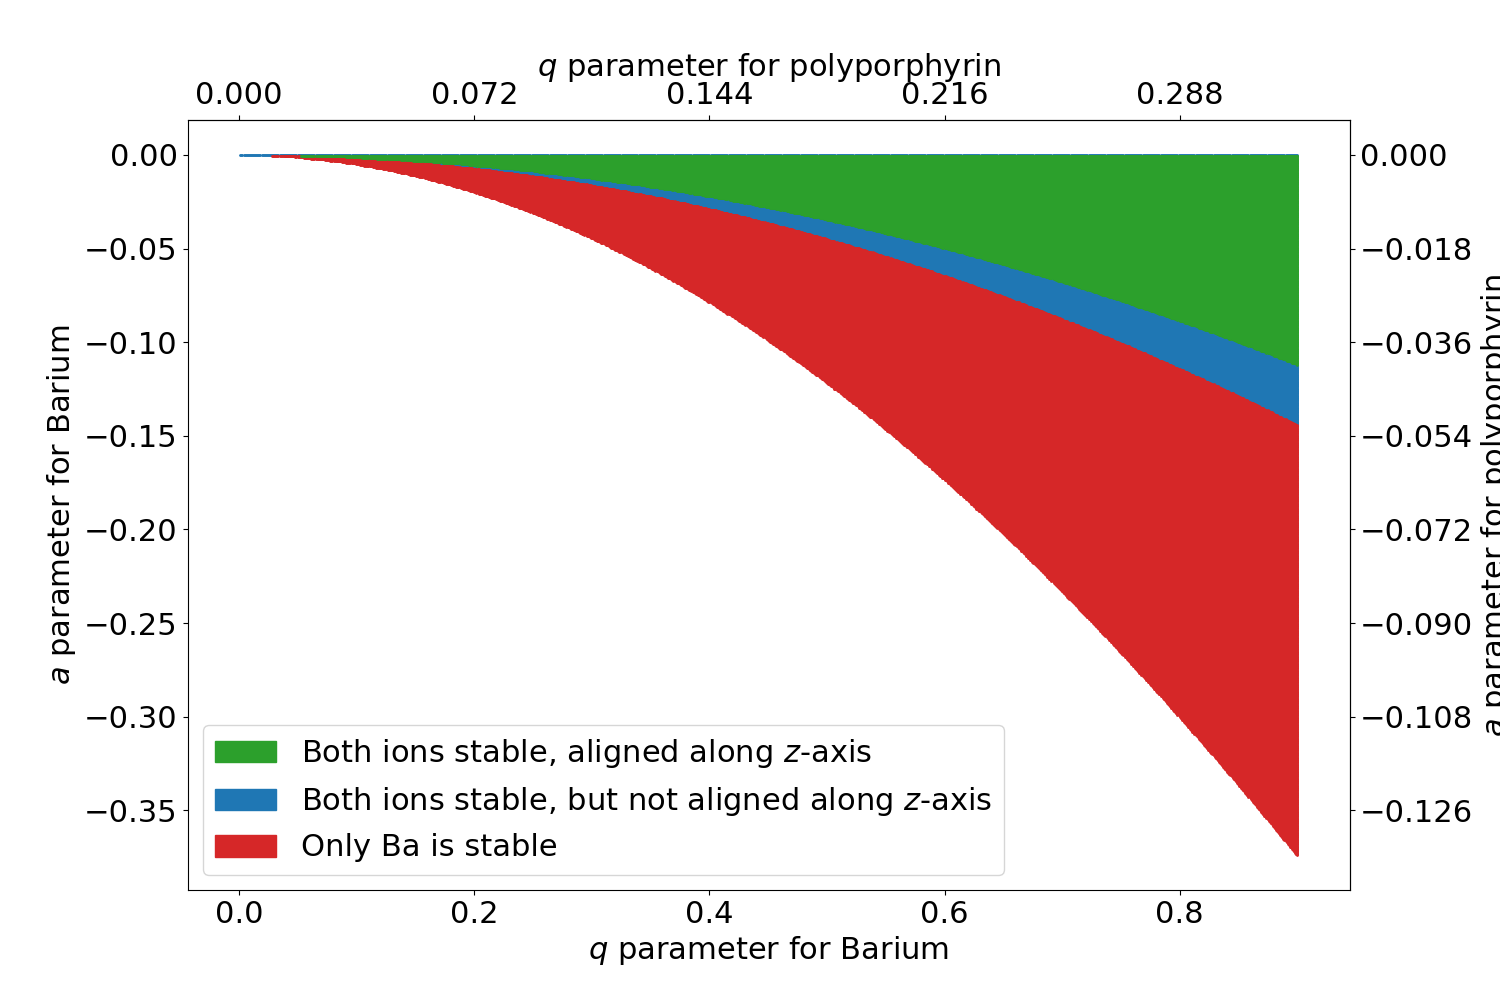
\includegraphics[width = \textwidth]{main/Stability2.png}
    \caption{Stability diagram for Ba$^+$ cotrapped alongside a polyporphyrin system, holding 12 porphyrin rings with 2 charges each for a total of $m_2 = 9000$amu, $Q_2 = 24$e. The green area represents the $a$ and $q$ parameters ideal for experiments as both ions have stable trajectories, while they also align along the $z$-axis.
    for trapping parameters that fall within the blue area the ions have stable trajectories, but will aliugn along the radial axes. Finally the red shaded area describes the parameters for which only the Ba$^+$ ion has stable trajectories. It is thus clear that trapping two ions with very different mass-to-charge ratios puts considerable additional bounds on the stability of the system.}
    \label{fig:Stability2}
\end{figure}


With the equilibrium positions of the ions, and the criteria for them to be stably trapped determined. One can now determine the new oscillation frequencies of the ions. To do this we reintroduce the full potential of \cref{eq:fullV} and perform a Taylor expansion to 2nd order around the equilibrium position of the system. When performing calculations of vibrational modes for coupled oscillators it is common to introduce mass-weighted displacement coordinates defined as
\begin{equation}
    \xi_1 = \sqrt{m_1}(z_{eq,1}-z_1),\quad \xi_2 = \sqrt{m_2}(z_{2,eq}-z_2),\quad \xi_3 = \sqrt{m_1}x_1,\quad \xi_4 = \sqrt{m_2}x_2.
\end{equation}
If we write up the Lagrangian for the system in this coordinate system we find
\begin{equation}
    \mathcal{L} = \sum_{i=1}^4 \dot{\xi}_i^2 - \frac{1}{2} \sum_{i = 1}^4K_{ij}\xi_i\xi_j,
\end{equation}
where $K_{ij} = \bigg(\frac{\partial^2 V}{\partial r_i\partial r_j}\bigg\vert_{eq}/\sqrt{m_im_j}\bigg)$ and $\{r_1,r_2,r_3,r_4\} = \{z_1,z_2,x_1,x_2\}$. It should be noted that the Taylor expansion in principle also adds an energy offset corresponding to the potential energy when the system is in equilibrium. We ignore this offset as it introduces no dynamics.

Explicit calculation of the $K_{ij}$ terms grants several zero's. The non-zero $K_{ij}$'s evaluate to
\begin{align}
    &K_{11} = \omega_{1,z}^2\bigg(1+\frac{2}{1+1/\rho}\bigg),\\
    &K_{12} = K_ {21} = -\frac{2\omega_{1,z}^2}{\sqrt{\mu}(1+1/\rho)},\\
    &K_{22} = \omega_{1,z}^2\frac{\rho}{\mu}\bigg(1+\frac{2}{1+\rho}\bigg),\\
    &K_{33} = \omega_{1,r}^2 - \frac{\omega_{1,z}^2}{1+1/\rho},\\
    &K_{34} = K_{43} = -\frac{1}{2}K_{12},\\
    &K_{44} = \omega_{2,r}^2-\frac{\omega_{1,z}^2}{\mu(1+1/\rho)}.
\end{align}
The coupled motional modes as well as their oscillation frequencies can now be found by diagonalizing the matrix \textcolor{red}{TAYLOR}
\begin{equation}
    K = \begin{bmatrix}
        K_{11} & K_{12} & 0 & 0\\
        K_{21} & K_{22} & 0 & 0\\
        0 & 0 & K_{33} & K_{34}\\
        0 & 0 & K_{43} & K_{44}\\
    \end{bmatrix},
\end{equation}
which is block diagonal. This simplifies the problem significantly, as it suffices to solve the eigenproblem for the two 2x2 matrices on the diagonal
\begin{equation}
    K_{z} = \begin{bmatrix}
        K_{11} & K_{12}\\
        K_{21} & K_{22}\\
    \end{bmatrix},
    \quad
    K_{r}
    \begin{bmatrix}
        K_{33} & K_{34}\\
        K_{43} & K_{44}\\,
    \end{bmatrix}
\end{equation}
which will give the solutions for the axial and radial motion respectively.
Solving the probem yields two modes for each direction, one where the ions move together in-phase with one another (sometimes referred to as the center-of-mass mode), and one where they move out of phase (sometimes referred to as the breathing mode).
For the frequencies one finds
\begin{align}
    &\big(\omega_z^{i/o}\big)^2 = \frac{K_{11}+K_{22}\mp\sqrt{(K_{11}-K_{22})^2+4K_{12}^2}}{2},\\
    &\big(\omega_r^{i/o}\big)^2 = \frac{K_{33}+K_{44}\pm\sqrt{(K_{33}-K_{44})^2+4K_{34}^2}}{2}.
\end{align}
Expanding the $K_{ij}$'s above would make the equations considerably harder to read, and as such is not done here. Denoting the normalized eigenmodes for the axial motion as $\vec{\alpha_{i/o}}$, and the ones for radial motion $\vec{\beta_{i/o}}$ one finds
\begin{align}
    &\vec{\alpha_{i/o}} = \frac{1}{\sqrt{1+\tilde{\alpha}_{i/o}^2}}
    \begin{pmatrix}
        \tilde{\alpha}_{i/o} \\
        1
    \end{pmatrix},\quad \tilde{\alpha}_{i/o} = \frac{\big(\omega_z^{i/o}\big)^2-K_{22}}{K_{12}},\\
    &\vec{\beta_{i/o}} = \frac{1}{\sqrt{1+\tilde{\beta}_{i/o}^2}}
    \begin{pmatrix}
        \tilde{\beta}_{i/o} \\
        1
    \end{pmatrix},\quad \tilde{\beta}_{i/o} = \frac{\big(\omega_r^{i/o}\big)^2-K_{44}}{K_{34}}.
\end{align}
Here the first component of the vector describes the amplitude, often referred to as the contribution or participation, of ion 1 in the motional mode, while the 2nd component of the vector describes the participation of ion 2.


For ions with very different charge-to-mass ratios one finds that the motion of the ions becomes essentially uncoupled. As an example we consider once again a Ba$^+$ ion trapped alongside a polyporphyrin ($m_2 = 9000$amu, $Q_2 = 24$e), here the axial eigenvector for the in-phase motion is $\vec{\alpha_{i}} = (0.092,0.99)$. Thus the in-phase motion of this system consists of almost exclusively motion of the heavy polyporphyrin. This decoupling of motion has significant consequences for cooling, as will be seen in \cref{chap:Cooling}.


Further expansion of the equations above makes them considerably harder to read, and thus is not done here. However, it is good to note that, roughly, one finds that $\tilde{\alpha}_{i/o}\propto\rho/\mu$, while $\tilde{\beta}_{i/o}\propto(\rho/\mu)^2$. This means the decoupling of the ion motion tends to be larger along the radial direction as the charge and mass ratios of the two ions become more skewed.
